\documentclass[12pt]{spieman}
\usepackage{amsmath,amsfonts,amssymb}
\usepackage{graphicx}
\usepackage{setspace}
\usepackage{tocloft}
\usepackage{lineno}
%\usepackage{amssymb}
\usepackage{multirow}
\usepackage{booktabs}
\DeclareMathOperator*{\argmin}{arg\,min} % thin space, limits underneath in displays
\newcommand{\bpm}{$\mathbf{\pm}$}
\newcommand{\second}{$^{\dag}$}
\newcommand{\best}{$^{*}$}
\graphicspath{{figures}}

\title{Self-supervised denoising of Nyquist sampled volumetric images via deep learning}

\author[a]{Matthew B. Applegate}
\author[b]{Kivanc Kose}
\author[a]{Sandesh Ghimire}
\author[b]{Milind Rajadhyaksha}
\author[a,*]{Jennifer Dy}
\affil[a]{Northeastern University, Department of Electrical and Computer Engineering, 360 Huntington Ave, Boston, MA, USA, 02115}
\affil[b]{Dermatology Service at Memorial Sloan Kettering Cancer Center, 530 E. 74th Street, New York, NY, USA, 10065}

\renewcommand{\cftdotsep}{\cftnodots}
\cftpagenumbersoff{figure}
\cftpagenumbersoff{table} 

\begin{document}
\maketitle
\linenumbers
%%%%%%%%%%%%%%%%%%% abstract %%%%%%%%%%%%%%%%
%% [use \begin{abstract*}...\end{abstract*} if exempt from copyright]
\begin{abstract}
\textbf{Significance:} Deep learning has demonstrated excellent performance enhancing noisy or degraded biomedical images. However, many of these models require access to a noise-free version of the images to provide supervision during training which limits their utility. Here, we develop a new algorithm (noise2Nyquist) that leverages the fact that Nyquist sampling provides guarantees about the maximum difference between adjacent slices in a volumetric image, which allows denoising to be performed without access to clean images. \textbf{Aim:} We aim to show that our method is more broadly applicable and more effective than other self-supervised denoising algorithms on real biomedical images, and provides comparable performance to algorithms that need clean images during training. \textbf{Approach:} We first provide a theoretical analysis of noise2Nyquist and an upper bound for denoising error based on sampling rate. We go on to demonstrate its effectiveness in denoising in a simulated example as well as real fluorescence confocal microscopy, computed tomography, and optical coherence tomography images. \textbf{Results:} We find that our method has better denoising performance than existing self-supervised methods and is applicable to datasets where clean versions are not available. Our method resulted in peak SNR (PSNR) within 1 dB and Structural Similarity Index (SSIM) within 0.02 of supervised methods. On medical images, it outperforms existing self-supervised methods by an average of 3 dB in PSNR and 0.1 in SSIM. \textbf{Conclusion:} Noise2Nyquist can be used to denoise any volumetric dataset sampled at at least the Nyquist rate making it useful for a wide variety of existing datasets.
\end{abstract}
% Include a list of up to six keywords after the abstract
\keywords{image enhancement, denoising, deep learning, self supervision}
% Include email contact information for corresponding author
{\noindent \footnotesize\textbf{*}Jennifer Dy,  \linkable{jdy@ece.neu.edu} }
\begin{spacing}{2}   % use double spacing for rest of manuscript

%%%%%%%%%%%%%%%%%%%%%%%%%%  body  %%%%%%%%%%%%%%%%%%%%%%%%%%

\section{Introduction}
Noise is nearly always a factor in any attempt to capture images of the world. Biomedical imaging is especially susceptible to noise because it often operates in regimes where signals are weak. In medical applications, noise can make images difficult for physicians to interpret and complicate diagnosis. Deep learning has recently proven to be a valuable tool for removing noise from biomedical images and revealing previously obscured structures\cite{Kaur2017}. Most common deep learning algorithms are supervised, meaning they require examples of noise-free data to effectively learn how to remove noise. While these techniques have demonstrated impressive performance, the need for images without noise for training limits their utility. In many biomedically relevant imaging modalities noise-free data is difficult or impossible to acquire.

Recently, self-supervised methods have been developed that are capable of denoising images without access to a co-registered noise-free version of the image during training. One method that has received widespread attention, called noise2noise, is able to learn the clean image given two noisy versions of the same underlying structure\cite{Lehtinen2018a}. One noisy image is used as the input to a neural network while the second is used as a target. During training, the network is unable to learn the random noise, so falls back to learning the underlying clean image. When such data are available, noise2noise has performance comparable to supervised methods, and has been applied for denoising retinal OCT images \cite{Huang2021,Huang2021a,Mao2019,Qiu2021}. The use of volumetric data for denoising has recently been explored\cite{Papkov2021}, but to date, this method has only been applied to MRI and, to the best of our knowledge, no analysis of the the impact of sampling rate has been undertaken.

In this manuscript, we will show how the noise2noise method can be extended to situations where the underlying structure in two images is similar, but not exactly the same. We call this method ``noise2Nyquist" because volumetric images collected at the Nyquist rate are guaranteed to have similar structure. Nyquist rate collection of volumetric data is common for methods such as optical sectioning microscopies and Optical Coherence Tomography (OCT). Relaxing the requirement of noise2noise that the underlying structure be identical significantly increases noise2Nyquist's utility over other methods, as our model relies neither on the existence of clean images, nor specialized acquisition techniques. Here, we show improved denoising performance over existing methods in fluorescence confocal images of flatworms, OCT images of skin, and low-dose abdominal CT images. 

Our contributions are the following: i) Development of a novel denoising algorithm for use on volumetric data. ii) Determination of the maximum error caused by using adjacent samples as a function of sampling rate. iii) Showing noise2Nyquist has superior performance relative to existing self-supervised machine learning and conventional image processing algorithms.

\section{Background}
The Nyquist sampling criterion states that image samples must be collected at at least twice the rate of the highest frequency in order to perfectly reconstruct the continuous signal\cite{Shannon1949}. In imaging, the maximum resolvable frequency of a modality is determined by the point spread function, which is the image formed by a structure smaller than the resolution limit of the instrument\cite{goodman2005introduction}. The point spread function provides information on the highest resolvable frequency, and thus the sampling rate required to preserve all information in the continuous image. Sampling at the Nyquist rate is common practice for most imaging modalities because lower rates can lead to aliasing of high-frequency signals, while higher rates increase storage demands without providing a resolution benefit. 

An ideal diffraction-limited point spread function is an Airy disk with a full-width at half maximum (FWHM) of $d_{\mbox{PSF}}=0.51\frac{\lambda}{NA}$, where $\lambda$ is the wavelength of light and $NA$ the numerical aperture of the objective. For two objects to be resolved according to the Rayleigh criterion they must be separated by at least $d_{\mbox{Ray}}=0.61\frac{\lambda}{NA}$ which, inverted, defines the maximum frequency in the image. Sampling at twice this frequency provides the Nyquist rate and, inverting again, gives the optimal distance between samples ($d_{\mbox{Nyq}} = d_{\mbox{Ray}}/2$). Dividing the Nyquist sampling distance by the Airy disk FWHM yields the sample separation as a function of the point spread function's width:

\begin{equation}
    \frac{d_{\mbox{Nyq}}}{d_{\mbox{PSF}}} = \frac{\frac{0.61\lambda}{2NA}}{\frac{0.51\lambda}{NA}} = \frac{0.61}{2\times0.51} \Rightarrow d_{\mbox{Nyq}}\approx0.6 d_{\mbox{PSF}}
    \label{eq:Nyquist}
\end{equation}

Equation \ref{eq:Nyquist} shows that, since $d_{\mbox{Nyq}} < d_{\mbox{PSF}}$. two adjacent pixels will have contributions from the same physical location on the sample. This relationship implies adjacent pixels in an image are guaranteed to originate, in part, from the same structure and, that neighboring frames of a volumetric image will be similar. Noise2Nyquist leverages this correlation between adjacent frames to extend noise2noise to the case where the two images have a similar, but not identical, underlying structure.

Since noise2Nyquist uses pairs of noisy images during training, it is theoretically similar to noise2noise which is described in detail by Lehtinen, et al.\cite{Lehtinen2018a}. Briefly, noise2noise uses multiple noisy images with the same underlying structure as both the input to and target of a neural network. The denoising problem is often constructed using the equation: $\hat{x}=x+n$ where $\hat{x}$ is the noisy image, $x$ is the unobserved clean image, and $n$ is the corrupting noise. The goal of the denoising algorithm is to find some function $f$ parameterized by $\Theta$ such that: $f_\Theta(\hat{x}) = x$. Lehtinen, et al. show that, so long as the corrupting noise is zero mean, the optimal parameters for the denoising network can be found by solving the risk minimization problem

\begin{equation}
	\argmin_\Theta \sum_i L(f_\Theta(\hat{y}_i),\hat{x}_i)
    \label{eq:riskMin}	
\end{equation}

where $L$ is a loss function, and both $\hat{x}_i$ and $\hat{y}_i$ are noise corrupted images of the same structure. If the noise is zero mean, the expected value of $\hat{x}_i$ given $\hat{y}_i$ is the unobserved clean image $x_i$. When $L$ in Equation~\ref{eq:riskMin} is the $L_2$ loss function, it will be minimized at the average of the images. If $L$ is the $L_1$ loss function, it will be minimized at the median of the images. This property allows us to find an upper bound the reconstruction error that could arise when images with a different underlying structure are used as the input to and target of a neural network during training. 

To explore this error, we used a 1-dimensional impulse as an illustrative example. We simulate imaging this structure by convolving the impulse with a Gaussian point spread function (Fig.~\ref{fig:noiselessSim}a). We then sampled the convolved signal at the Nyquist frequency, calculated using Equation~\ref{eq:Nyquist}, to generate a simulated image. Using this example, we are able to estimate the reconstruction error of noise2Nyquist using $L_2$ loss by taking a 3-point moving average of the simulated image, and, similarly, error using the $L_1$ loss function by taking a 3-point moving median. The plots in Fig~\ref{fig:noiselessSim} represent expected values of the functions and won't change in the presence of zero mean noise in the limit of infinite data.

We found the error when recovering an image of a point with an $L_1$ loss function depended on where the point fell relative to the image samples. When a sample fell exactly at the true location of the point, the error was maximized at 62\% (Fig.~\ref{fig:noiselessSim}b). When the imaged point fell at the midpoint between samples, the running median was identical to the true image yielding an error of 0\% (Fig.~\ref{fig:noiselessSim}a). The $L_2$ case, simulated by a running average, was less sensitive to the location of the point relative to the samples. The maximum error was 42\% when the point was located at the midpoint between two samples. The error was minimized at 22\% when the point fell at a sampled location. The finite bandwidth imposed by the imaging system, along with Nyquist sampling, bounds the reconstruction error of this method. 
The point-by-point error is arguably less important than the shape of a Gaussian curve fit to the data which is a common definition of resolution. To determine how sampling density affects the reconstructed image of a point, we varied it between 0.5 and 3 times the Nyquist frequency. For each sampling density, we varied the location of the samples relative to the point and fit a Gaussian function to the running average and running median. Using this fit, we were able to measure how the width of the reconstructed image changed by plotting the largest and smallest width at every sampling density (Fig.~\ref{fig:noiselessSim}d). We found that the difference between the maximum (solid lines) and minimum (dashed lines) error was very small when an $L_2$ loss function was used which indicated an insensitivity to the position of the point relative to the samples. The $L_1$ loss function, on the other hand, was very sensitive to the location of the point with error values ranging from about 0 to almost 3 times the true width. Comparing the two curves, we found that that the $L_1$ loss function always had a value closer to the true point spread function width than the $L_2$ loss function. Furthermore, Fig.~\ref{fig:noiselessSim}d shows that the Nyquist frequency is located at a corner on the PSF width curve which indicates that sampling at frequencies lower than the Nyquist rate resulted in the possibility for very large errors, while sampling higher than the Nyquist rate provided diminishing returns on performance. At the Nyquist frequency, the width of the image of the point was about 1.7 times larger when an $L_2$ loss was used, while for $L_1$ loss the standard deviation varies between 0 and 1.5 times larger depending on where the point fell relative to the samples.

We performed the same analysis when the structure was an edge instead of a point (Fig.~\ref{fig:noiselessSim}c). In this case, we found the error between the true image (orange solid line), and the simulated noise2Nyquist solution using an $L_2$ loss function (green circles) or an $L_1$ loss function (red tri-point), was calculated for each sample. We found the maximum error in the reconstructed image would be about 12\% when using $L_2$ loss, and 0\% when using $L_1$ loss. We also found that the edge was broadened by two samples relative to the ideal image when using $L_2$ loss. 

The simulation here was performed under noise-free conditions so all errors can be attributed to the use of adjacent pixels for reconstruction. The noise2noise algorithm requires multiple samples at the same physical location so would have perfect reconstruction in the noise free case. For both the algorithms, the presence of noise will affect the accuracy of the reconstruction.

While the maximum errors associated with noise2Nyquist can be relatively large, it is worth noting that this is an upper bound that only applies to the worst case scenario where the signal from a sub-resolution structure jumps from 0 to saturation and is located close to the center of a pixel. Most images are much more slowly varying leading to errors that are, in practice, much smaller. 

\begin{figure}[hbt]
	\begin{center}
		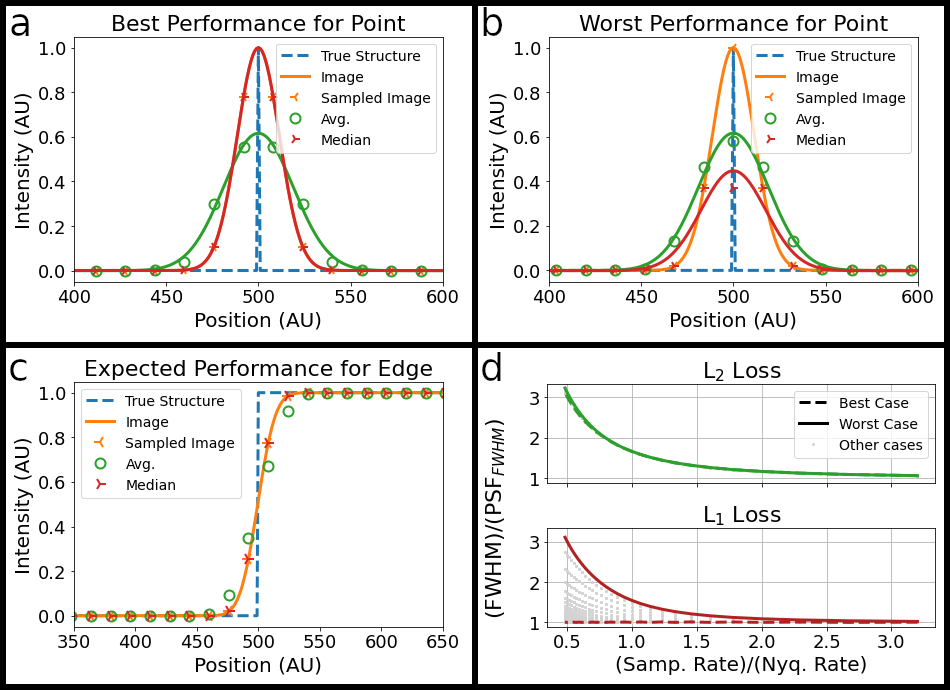
\includegraphics[width=0.5\textwidth]{noNoiseSimulation_ver02}
		\caption{\label{fig:noiselessSim} Simulated error due to the use of two adjacent pixels when training a neural network. a) Best performance when reconstructing an image of a point. Lines connecting Avg. and Median points are best fit Gaussian curves. b) Worst performance when reconstructing an image of a point. c) Reconstruction of an edge using running mean and running median data points. d) Plot of the reconstructed point spread function standard deviation under different loss functions and sampling rates. Solid lines indicate the best case location of the point relative to the samples, and dashed lines indicate the worst case. Other calculated PSF widths are shown as gray points. A value of 1 indicates no error. }
	\end{center}
\end{figure}

\section{Methods}
Our goal was to test the feasibility of denoising a variety of biomedical images by using adjacent frames of an image stack as inputs to and targets of a neural network. This section will describe the neural network, details of the training, data sources, and the evaluation metrics considered.

\subsection{Data}

We first used simulated data to assess the ability of our algorithm to remove noise. We used two model datasets: a standard Shepp-Logan phantom \cite{Shepp1974}, and a modified Shepp Logan phantom developed by Yu, et al.\cite{Yu2004} both of which simulate CT images of a head containing ellipsoidal inclusions. First, a high-resolution version of the phantoms consisting of 512x512x512 voxels was generated. This phantom was convolved with a 3D isotropic Gaussian function to generate the noise-free image and converted to 8-bit grayscale values. These ideal images were then sampled at various rates along one axis to simulate different sampling regimes (i.e. Nyquist or sub-Nyquist sampling). The sampled images were then corrupted by zero mean additive white Gaussian noise with a standard deviation of 45 ($\sim$18\% of the maximum signal value). All training was done on the Shepp-Logan phantom, and all testing was done on the Yu phantom.

We also gathered a variety of biomedical imaging data from different imaging modalities and biological structures to assess the performance of our denoising method. For all modalities we split the data on the patient level when available and on the volume level when not into 10 non-overlapping folds and report results from the test set in all cases.

We used a confocal fluorescence microscopy dataset from a recent study \cite{Weigert2018b}, where the authors collected 16-bit images of Planaria whose nuclei were stained with RedDot1 near infrared dye. The dataset consisted of 16 volumes with 95 slices of 1024 x 1024 pixel images. Co-registered images were collected with both low and high laser power. The low laser power images had significant noise while the high power images had much better quality. Images were split into 64x64 pixel patches with an overlap of 32 pixels. Many of the images had large background regions with no nuclei. To avoid training excessively on those regions, only patches with a Shannon entropy higher than 11 were considered. This cutoff value was chosen by qualitatively assessing the patches and choosing a value that excluded those containing few nuclei. We follow \cite{Weigert2018b} and normalize each image between 0 and 1 using the 0.1 and 99.9th percentile pixel values. For the clean images, the minimum value of the 99.9th percentile was set to 25,000 to avoid amplifying noise. Noisy images were normalized using the 2nd and 99.7th percentile values. We obtained a total of 123,452 noisy/clean image patches using this method. We followed the method of Weigert et al.\cite{Weigert2018b} to ensure the denoised and clean data were comparable by affinity scaling. Each noisy patch was linearly scaled to minimize the mean squared error between the clean and denoised images prior to evaluation. 

The second dataset that we used in this study was composed of X-ray computed tomography (CT) images from the Mayo Clinic 2016 low-dose CT Grand Challenge\cite{McCollough2017}. This dataset consisted of CT data from 10 patients with suspected metastatic liver lesions imaged using the standard radiation dose. These clean images were corrupted with noise to simulate low-dose measurements from the same patients. We used the 16-bit images that were reconstructed with the standard Siemens B30 kernel for soft tissue with 1 mm spacing between slices. This resulted in about 500 512x512 pixel slices per patient. These data were split into 64x64 pixel patches with 32 pixel overlap. To avoid images consisting only of background, we only considered the roughly 5\% of patches with the highest Shannon entropy, leading to a cutoff value of 9. The same affinity scaling was used as the fluorescence confocal data to allow us to make comparisons between denoised and clean images. We obtained a total of 76,143 paired low-dose/high-dose patches using this method. 

Finally, we tested our denoising strategy on a dataset collected in our lab. This dataset contained optical coherence tomography (OCT) images from 36 patients with skin lesions suspicious for basal cell carcinoma. The data were collected on living patients and consisted of 490 B-scans each of 512x245 pixels sampled at the Nyquist rate in all dimensions\cite{Iftimia2017a}. The frames were split into 64x64 pixel patches. To avoid patches containing solely background signal, only 25\% of patches with the highest Shannon entropy were included. The entropy cutoff for this dataset was 7. After pre-processing, this dataset consisted of a total of 391,182 patches. 

\subsection{Algorithms}
We compared the performance of noise2Nyquist against several other deep learning and conventional denoising methods to highlight its utility. When clean versions of the images were available we used a supervised approach that trains a neural network with a loss function comparing the output image to the ground truth. For our simulated phantom we were able to produce multiple noisy versions of each slice so were able to compare our method to the noise2noise technique described above. We also used another popular self-supervised denoising method called noise2void\cite{Krull2019} which uses a mask based approach to estimate noise-free pixel values from neighboring pixels, and so does not require paired or noise-free images. We also compared noise2Nyquist with a newer technique, neighbor2neighbor, that uses subsampling to generate pairs of noisy images\cite{Huang2021b}. These image pairs can be used for denoising in a manner similar to noise2noise, but with an added regularization term to account for differences between the two images. Recent supervised video denoising methods such as Mu-Net\cite{Lee2020a}, ViDeNN\cite{Claus2019}, and Fastdvdnet\cite{Tassano2020} leverage adjacent video frames for denoising like noise2Nyquist, but require clean versions of the image stack during training, so cannot be used when only noisy data are available.

We also compared noise2Nyquist to several conventional image processing tools. We tested a median filter with a 3x3 window size and a Gaussian blurring kernel with a standard deviation of 1 pixel. We also investigated taking the average of 3 sequential frames which is commonly used to denoise volumetric images. Finally, we investigated two more complex algorithms: Block matching and 3D filtering (BM3D) which is used for single images\cite{Dabov2007} and it's volumetric extension block-matching 4D (BM4D)\cite{Maggioni2013}. When evaluating the BM4D method stacks of 3 images were used to be comparable with the out of frame averaging and machine learning methods. Both BM3D and BM4D have shown excellent denoising performance across a wide variety of data, but are computationally complex and therefore prohibitively slow for many applications.

\subsection{Neural network}
We tested the machine learning denoising methods using the U-Net network described in Ref.~\cite{Lehtinen2018a} (Fig.~\ref{fig:netStructure}). It consisted of an encoder with 5 stages where the size of the input was reduced by half at each stage. Each encoder stage consisted of a convolutional layer with 48 filters and a 3x3 filter size, followed by a rectified linear unit (ReLU) activation layer, and a 2d max pool layer. The encoder of the U-Net was followed by a decoder also consisting of 5 stages. During each stage of decoding, the output of the corresponding encoder stage was concatenated to the input of the decoding stage. These skip connections have been shown to reduce problems due to vanishing gradients and improve performance\cite{He_2016_CVPR}. Each decoding stage consisted of a convolutional layer with 48 channels plus the number of channels from the corresponding encoder stage with 3x3 filters. The convolutional layer was followed by a ReLU layer, a second convolutional layer, and a second ReLU layer. Finally, a 2D transposed convolutional layer with a stride of 2 was used to increase the size of the output. The final model consisted of 698,017 trainable parameters.

\begin{figure}[htb]
	\begin{center}
	\includegraphics[width=0.5\textwidth]{networkStructure}
	\caption{\label{fig:netStructure}Network structure used to evaluate the performance of medical imaging denoising.}
	\end{center}
\end{figure}

\subsection{Training}

The networks were trained on a 65,536 random samples from within each training split. Input data were normalized by subtracting the mean and dividing by the standard deviation of the entire training set. We used random vertical and horizontal flipping of each minibatch to augment training data. During training, a patch from the training set would be randomly selected for consideration. The patch co-located at the preceding, or the following frame would be randomly selected for use as the comparison. Which frame was used as input and which used as the target was also randomly selected for each mini-batch. For phantom training, a batch size of 4 was used, while a batch size of 64 was used for all other datasets. Each model was trained for 150 epochs. An ADAM optimizer with an initial learning rate of 0.001 was used with betas of 0.9 and 0.99 \cite{Kingma2015}. The learning rate was decreased each epoch using an exponential rate decay with a gamma constant of 0.97. Each fold took about 4.5 hours to train on a single NVidia RTX 3060 GPU.

\subsection{Evaluation Metrics}
When co-registered clean images were available, three metrics were used to assess denoising quality: peak signal-to-noise ratio (PSNR), Structural Similarity Index (SSIM)\cite{Wang2002}, and Mean Squared Error (MSE). MSE is a pixel-wise error metric that compares the values of pixels in the candidate image, with the values in the reference image. It is defined as $\frac{1}{mn} \sum_{i=0}^m\sum_{j=0}^n(I(i,j) - K(i,j))^2$. Where $I$ and $K$ are the reference and candidate image respectively, and $m$ and $n$ are the image height and width. PSNR can be written as $20\cdot\log_{10}(MAX/\sqrt{MSE})$. Where $MAX$ is the maximum possible pixel value for the image bit depth and $MSE$ is the mean squared error between the reference and candidate image. SSIM takes into account components of the human visual system to obtain a metric of image quality that ranges from 0 to 1. It is defined as
\begin{equation}
	SSIM(I,K) = \frac{(2\mu_I\mu_K + c_1)(2\sigma_{IK}+c_2)}{(\mu_I^2 + \mu_K^2 + c_1)(\sigma_I^2 + \sigma_K^2 + c_2)}
\end{equation}
Where $\mu_x$ is the average of image $x$, $\sigma_x$ is the variance of image $x$, and $\sigma_{xy}$ is the covariance between images $x$ and $y$. Constants $c_1$ and $c_2$ are small constants ($c_1$=6.5 and $c_2$=58.5 in this implementation) to stabilize the equation when the denominator is small. We used PSNR and SSIM functions from the scikit-image Python package\footnote{https://scikit-image.org/}. For these metrics, high values of PSNR and SSIM indicate good denoising performance, while low values of MSE are desirable. 

The OCT dataset images were collected using a standard imaging protocol so there were no clean versions to assess the quality of denoising against. For these images, we use the Natural Image Quality Index (NIQI), a reference-free image quality assessment to quantify the success of the denoising algorithms\cite{Mittal2013}.

These metrics seek to quantify image quality, but they are imperfect. Images that score highly can contain unacceptable artifacts, while low scoring images can be the result of imperceptible differences such as a small offset at every pixel. Better methods such as expert reader evaluations are beyond the scope of this manuscript, but will be included in future work.

\section{Results}

The following sections will present the denoising results on simulations and a variety of different medical imaging modalities. A summary of all results is shown in Table~\ref{tab:allresults}. All of the data presented here are from the test set of the models meaning that the metrics were calculated from data that had not been seen by the network during training. The 10 fold cross validation ensures that every volume appeared in the test set of one of the folds allowing this analysis to be performed. However, one benefit of self-supervised methods is that the risk of over training is reduced and there is no way for the model to ``memorize" the clean training dataset. If sufficient data are available, it is possible to train these models directly on the data to be denoised which would avoid some sources of error and potentially yield better results.

\subsection{Phantom}
Results from processing the simulated data are shown in Fig.~\ref{fig:phantomResults}. The supervised, noise2noise, noise2void, and noise2Nyquist methods look visually quite similar. As the sampling rate in the Z-direction is decreased, the noise2Nyquist reconstructed image degraded. The other methods, since they do not take information from adjacent frames, are unaffected by the sampling rate. The structural similarity index in Fig~\ref{fig:phantomResults}i showed that the supervised, noise2noise, and noise2nyquist methods have essentially identical metrics following training so long as sampling is performed at at least the Nyquist rate. As the sampling rate goes down, the SSIM decreases from an average of 0.96 to an average of 0.88. These observations are echoed in the plot of MSE (Fig~\ref{fig:phantomResults}j) which show the same trends. PSNR (not shown) was similar to the inverse of MSE as expected from the definition. When the sampling rate is reduced there is no longer a guarantee that adjacent slices arise from the same physical location which may lead the model to learn unexpected structures which can reduce performance. The neighbor2neighbor algorithm (see Table~\ref{tab:allresults} performed surprisingly poorly on this dataset with an average SSIM of 0.74 and average PSNR of 26.9 dB.
\begin{figure*}[htb]
	\begin{center}
		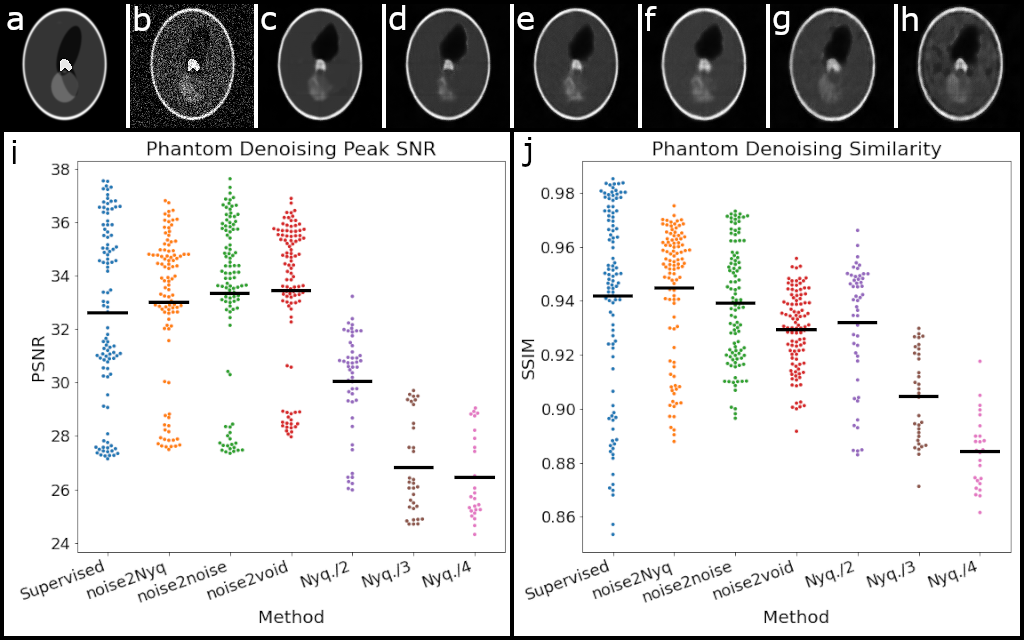
\includegraphics[width=.8\textwidth]{phantomResults_Horiz_ver02}
		\caption{\label{fig:phantomResults}Denoising results using various methods on simulated data. a) Clean image b) Noisy image c) Supervised d) Noise2noise e) Noise2void f) Noise2Nyquist (ours) g) Noise2Nyquist with a Z-sampling rate of half the Nyquist rate h) Noise2Nyquist with a Z-sampling rate of one quarter the Nyquist rate. i) Swarm plot of the Structural Similarity Index (SSIM) for different denoising methods. Horizontal bar indicates the mean. j) Swarm plot of the mean squared error (MSE) for different methods.}
	\end{center}
\end{figure*}

\subsection{Fluorescence Confocal}
Confocal images were denoised with 4 different ML methods: the supervised method that required a clean version of the image to use during training, our method, noise2Nyquist, that used adjacent images from only the noisy volumes, and noise2Void and neighbor2neighbor which denoised each frame independently without clean data. Fig.~\ref{fig:confocalResults} (left) shows a typical example of the images used in this experiment. The clean version (a) was collected at high laser power, while the noisy version (b) was collected at lower power. These images show that the supervised method (c) and noise2Nyquist (d) produce similar looking results despite the fact that noise2Nyquist does not require a clean image during training. The noise2void method (e) removed the random component of the noise, but left structured noise in the final image. Neighbor2neighbor (f) effectively removed the noise, but the nuclei showed increased structure not found in the clean version of the image. Quantitative results are shown for the image quality metrics described above in Fig.~\ref{fig:confocalResults}. Panel g shows violin plots for 1536 patches from four of the 16 total volumes investigated. They illustrate that the quality of the denoising varies across volumes. However, there is a general trend of the supervised and noise2Nyquist method providing roughly equivalent performance. Noise2void performed worse due to the presence of structured noise which cannot be removed by this method. Neighbor2neighbor had better performance than noise2void, but worse performance than either the supervised method or noise2Nyquist. Panel h shows boxplots of the metrics across all denoised frames. This plot echoes the plot above showing that the supervised method performs slightly better than noise2Nyquist, with noise2void and neighbor2neighbor performing less well.
\begin{figure*}[htb]
	\begin{center}
		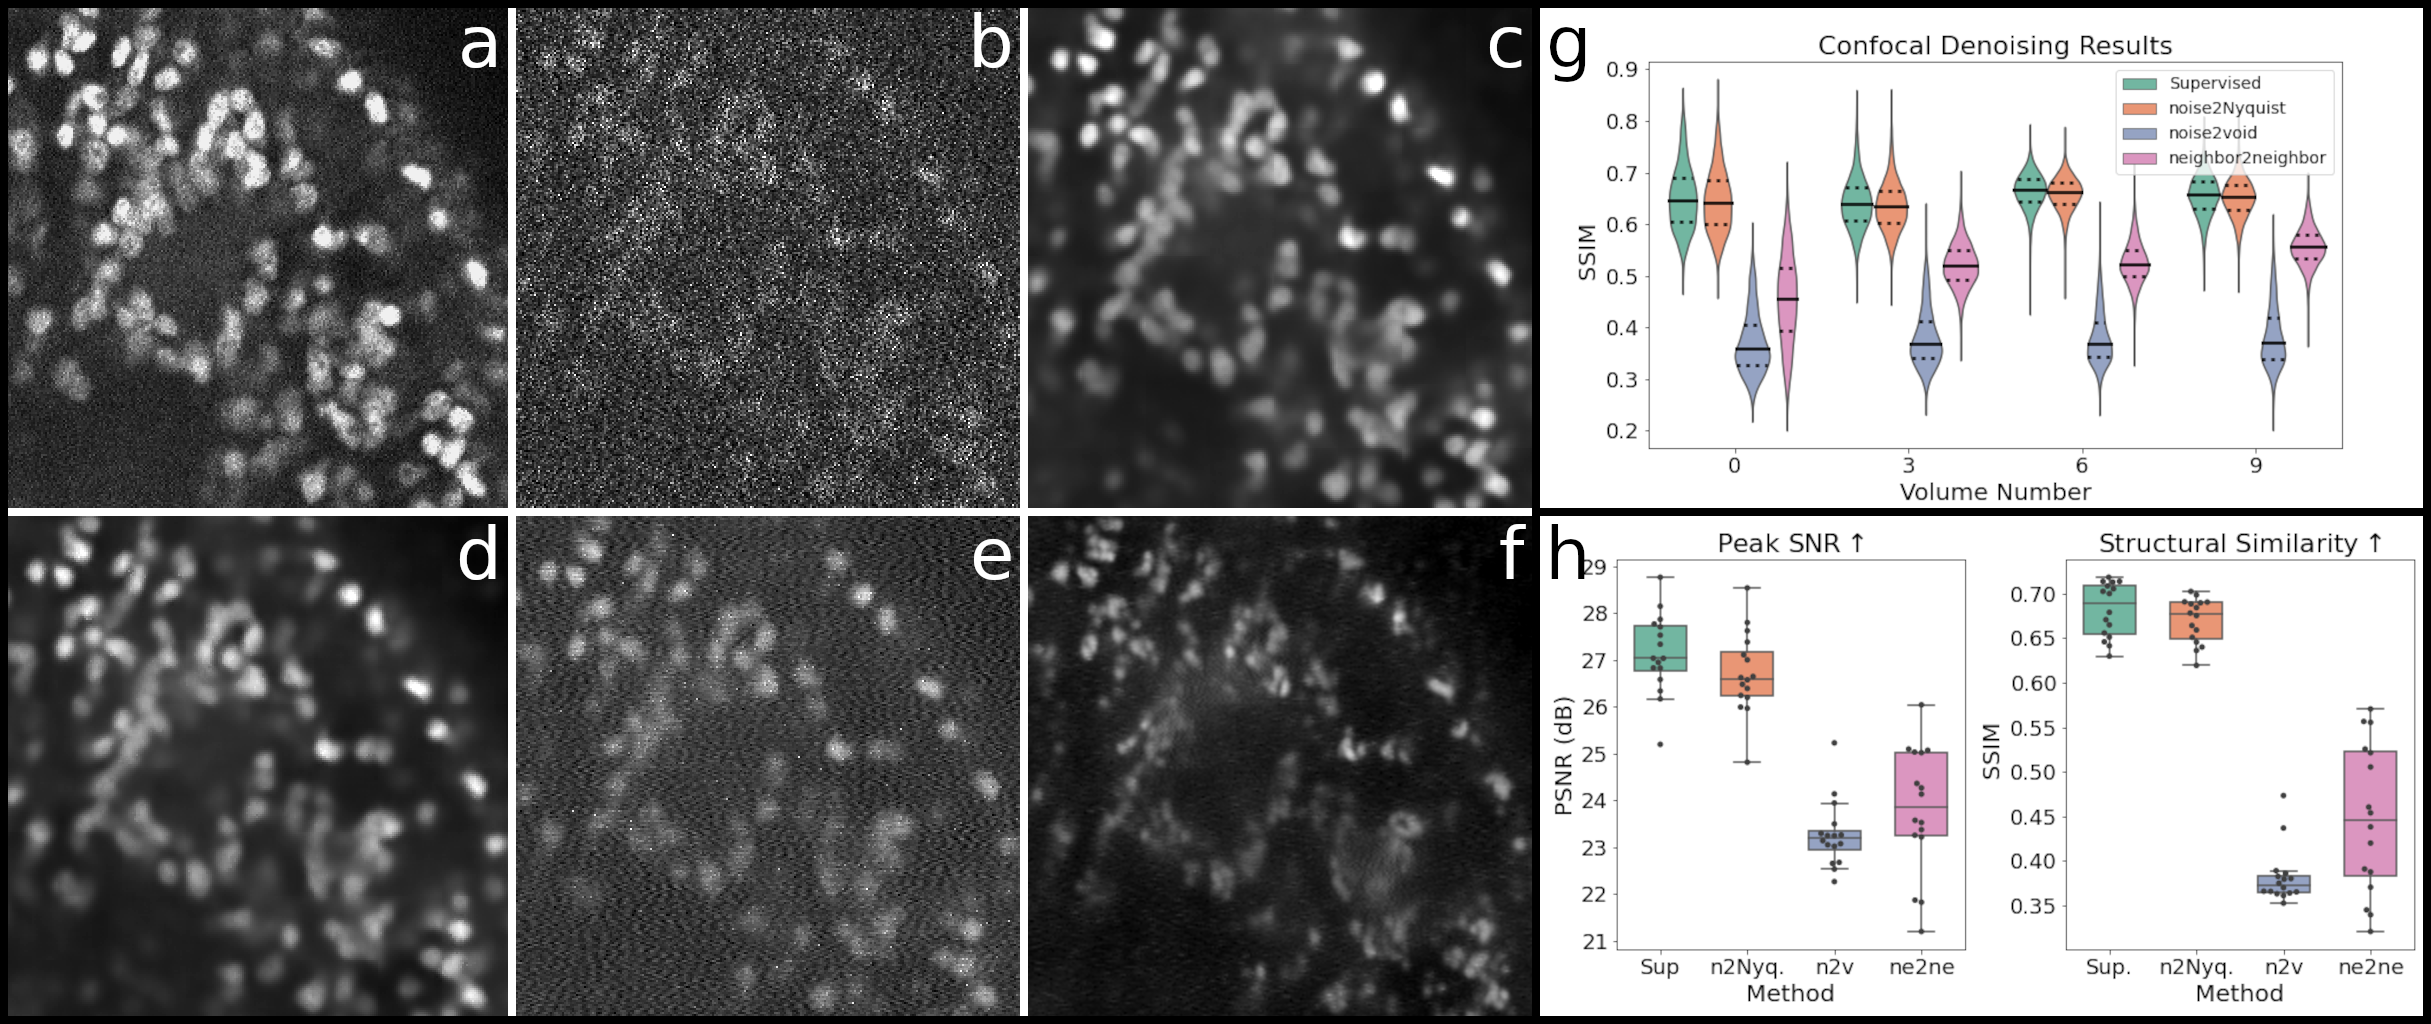
\includegraphics[width=\textwidth]{confocalFig_ver04}
		\caption{\label{fig:confocalResults}Left) Example fluorescence confocal denoising performance. a) Clean image b) Noisy image c) Supervised  d) Noise2Nyquist (ours) e) Noise2void f) Neighbor2neighbor g) Structural similarity index violin plot for 1536 64x64 pixel patches from representative volumes. Solid lines represent the median values. Dotted lines show the 25th and 75th percentile. h) Boxplots showing average denoising performance over all volumes. Arrows in title indicate which direction represents closer match to clean image. Each gray datapoint overlayed on the boxes is the average of 1536 patches from a single volume. ``ne2ne" stands for the ``neighbor2neighbor" method.}
	\end{center}
\end{figure*}

\subsection{Computed Tomography}
The computed tomography dataset was denoised with the same methods as the confocal images and the results are shown in Fig.~\ref{fig:ctResults}. Visually, the supervised version appeared to be oversmoothed compared to the ground truth. The noise2Nyquist results retained much of the image texture found in the clean version of the image. The noise2void and neighbor2neighbor methods were not very successful for this dataset leading to images that looked more similar to the noisy image than the clean. The supervised, noise2Nyquist, and BM4D processed images all make it easier to spot the tumor indicated by the white arrows in Fig.~\ref{fig:ctResults}a-f. However, the use of BM4D resulted in artifacts that have similar morphology to liver metastases (panel f, red arrows) that may cause confusion during diagnosis. Panel c shows some artifacts due to the patch-based processing that could be eliminated by considering patches with additional overlap. Panel g shows the SSIM for 256 randomly selected frames from 4 volumes. On this metric the supervised algorithm and noise2Nyquist performed similarly. Panel h shows boxplots for the average metric value across all patients. For PSNR our noise2Nyquist method performed the best of all the methods investigated. It tied the supervised algorithm for best performance on SSIM.

\begin{figure*}[htb]
	\begin{center}
		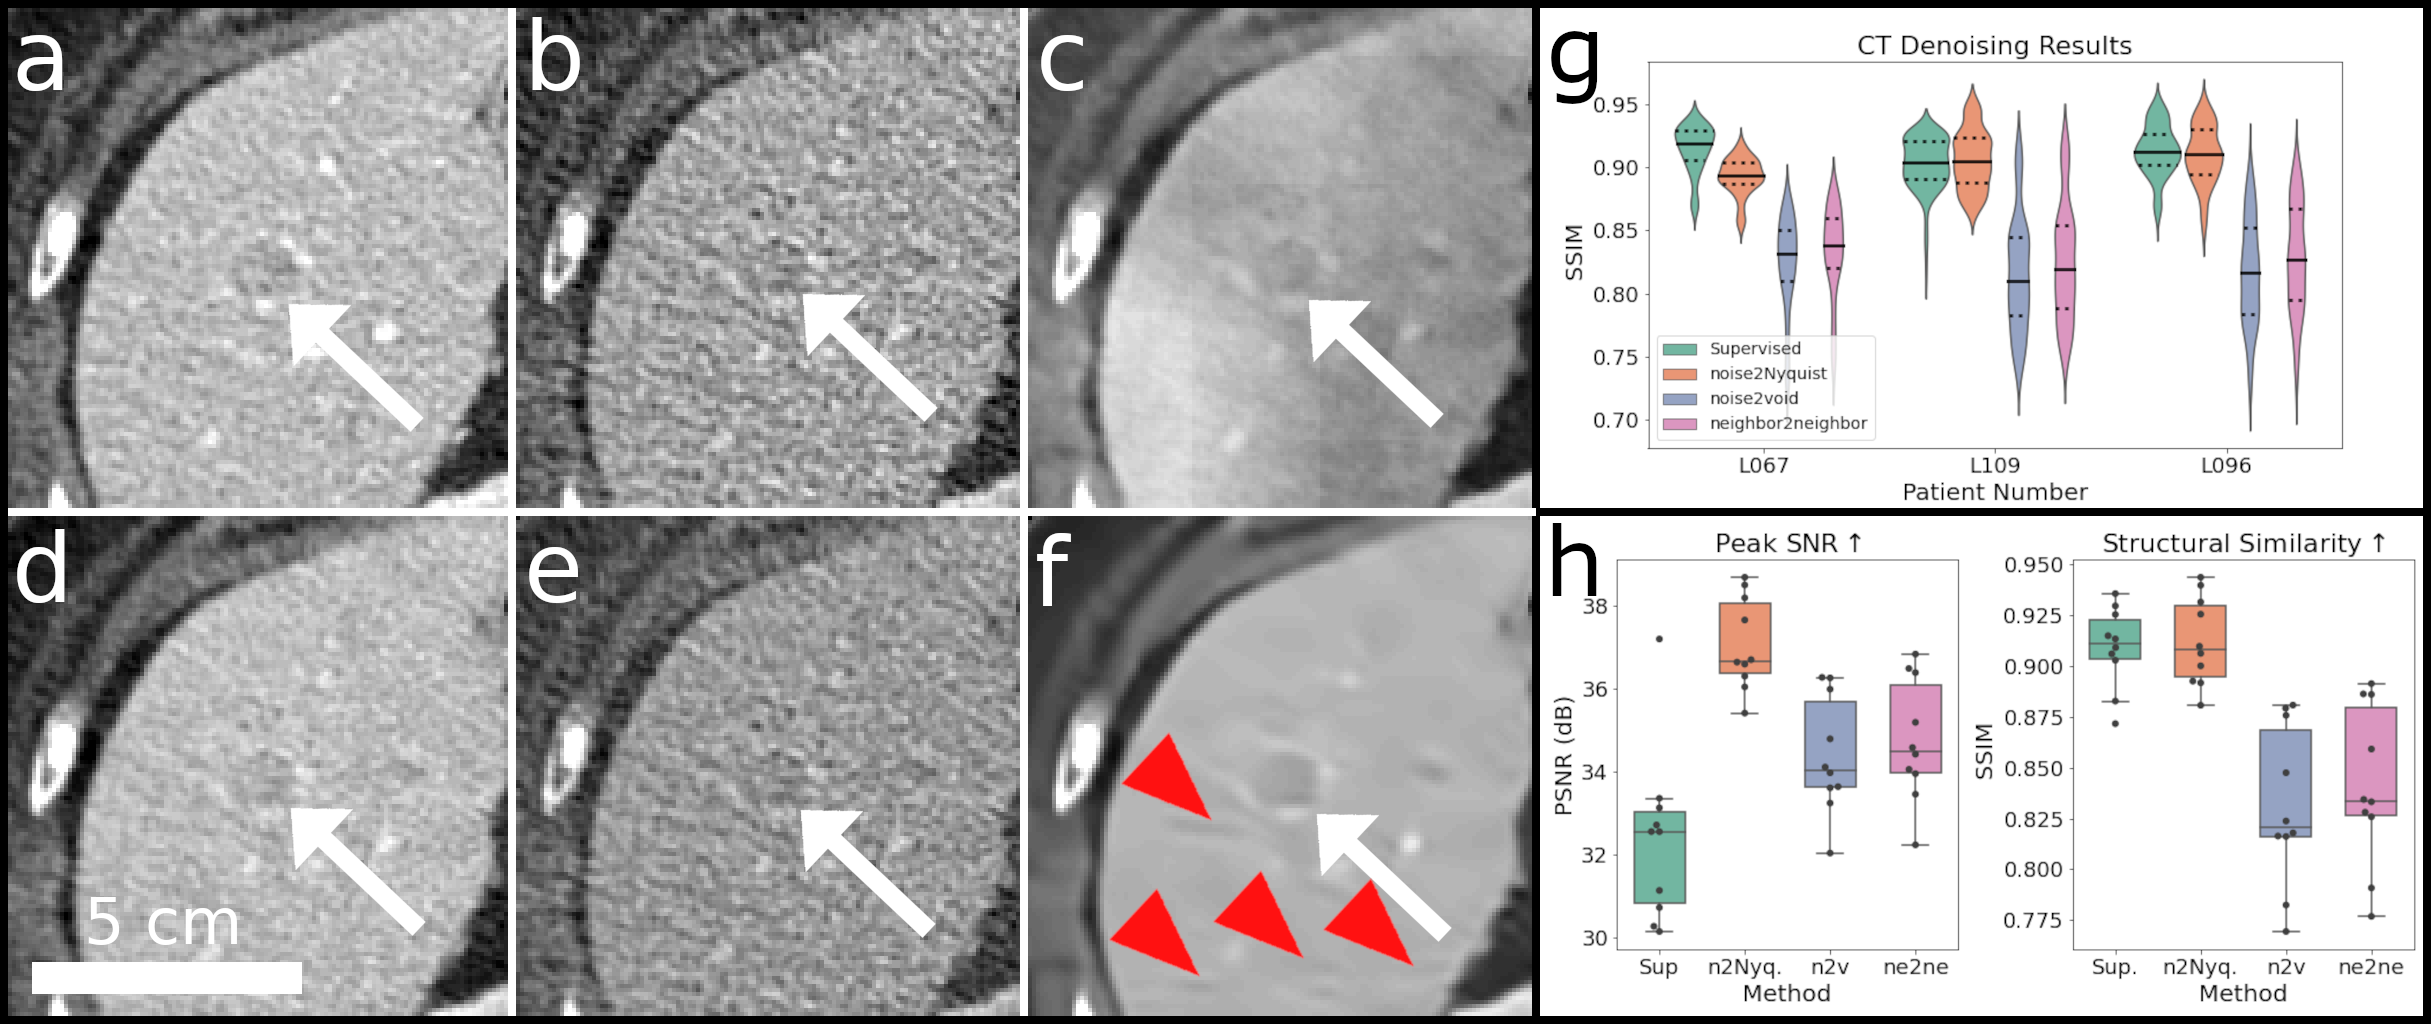
\includegraphics[width=\textwidth]{CTDenoisingFigure_ver03}
		\caption{\label{fig:ctResults}Example CT images a) clean b) noisy c) Supervised d) noise2Nyquist (ours) e) noise2void f) BM4D. White arrows indicate a metastatic liver lesion. Red triangles point to potentially misleading artifacts. Scale bar applies to all images. g) Violin plots of SSIM for representative patient scans based on 256 random frames. Dotted lines show the 25th and 75th percentile, solid lines show the median value h) Boxplots showing average denoising performance over all patients. Arrows in title indicate which direction represents closer match to clean image. Each gray datapoint overlayed on the boxes is the average of 256 random frames from a single patient. Ne2Ne stands for neighbor2neighbor.}
	\end{center}
\end{figure*}

\subsection{Optical Coherence Tomography}

The optical coherence tomography dataset was collected with a combined OCT and RCM device\cite{Iftimia2017a} using standard protocols, so do not include a co-registered clean image. Because of this, we were not able to use supervised methods. The lack of a clean image also make it impossible to use standard image metrics such as PSNR and SSIM. Instead, we chose to use the Naturalness Image Quality Index described above. Qualitatively, images trained using our noise2Nyquist method are much smoother and easier to interpret than the original images or those processed with noise2void, neighbor2neighbor, or conventional methods (Fig.~\ref{fig:octResults}a-f). Noise2void left behind structured noise which interfered with the appreciation of tissue morphology. Neighbor2neighbor left behind some speckle noise, but is marginally smoother than noise2noise. Tissue morphology in images processed with noise2Nyquist was more clear than in out of frame averaging and images processed with BM4D. Quantitatively, we found that the NIQI was much better for noise2Nyquist than noise2void and neighbor2neighbor. Panel g shows violin plots of the change in NIQI for 96 frames. The data are presented as the NIQI of the denoised image divided by the NIQI of the original image. Values lower than 1 indicate improvement in the image naturalness. The noise2Nyquist method resulted in values below 1 for all patients, while some patients processed with the noise2void and neighbor2neighbor methods had values greater than 1. Panel h shows aggregate NIQI for the 96 frames from all the patient scans. These results indicate that noise2Nyquist consistently outperformed noise2void and neighbor2neighbor for this dataset.

\begin{figure*}[htb]
	\begin{center}
		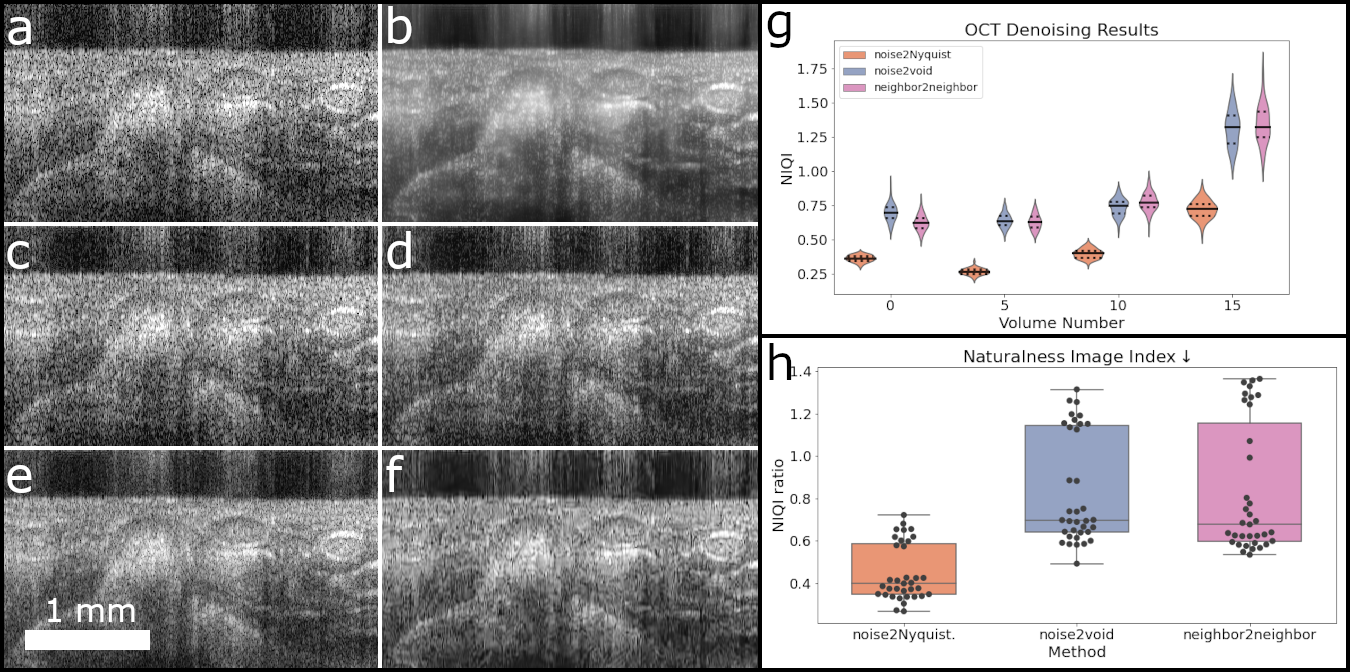
\includegraphics[width=\textwidth]{octResultsFigure_ver03}
		\caption{\label{fig:octResults}Representative images from volume 15. a) Original b) noise2Nyquist (ours) c) noise2void d) neighbor2neighbor e) 3 frame average f) BM4D. g) Violin plots showing the distribution of NIQI ratio for 7 volumes. Each violin represents 96 images. Dotted lines show the 25th and 75th percentile. Solid line shows the median value. Values below 1 indicate improvement on this metric. h) Boxplots showing average NIQI ratio over all volumes. Each gray datapoint overlaid on the boxes is the average of 96 Images from a single volume. The arrow in the title indicates lower values are better according to this metric.}
	\end{center}
\end{figure*}

\begin{table*}[htb]
\caption{\label{tab:allresults} Metrics from all tested methods. Values are presented as the mean of all volumes in the dataset plus or minus one standard deviation. A ``--" is used when sufficient data were not available for a particular method. Best scores are indicated with \best. Second best scores are indicated with \second.}
\begin{center}
    \resizebox{\textwidth}{!}{%
	\begin{tabular}{rccccccc}
	\toprule
		\multirow{2}{*}{\vspace{-2.5em}Method\hspace{1.5em}} &
		\multicolumn{2}{c}{Phantom}&
		\multicolumn{2}{c}{Fluo. Confocal} &
		\multicolumn{2}{c}{CT} &
		OCT  \\
		\cmidrule{2-8} 
		& PSNR & SSIM  & PSNR & SSIM  & PSNR & SSIM  & NIQI  \\
		\midrule
		Noisy & 17.14$\pm$0.01 & 0.166$\pm$0 & 11$\pm$2 & 0.06$\pm$0.02 & 34$\pm$2 & 0.82$\pm$0.06 & 1 \\		
		Supervised & 33.4\bpm0.3\best & 0.945$\pm$0.001\best & 27.1\bpm0.8\best & 0.68\bpm0.03\best & 32$\pm$2 & 0.91$\pm$0.02\second & -- \\
		Noise2Nyquist (ours) & 32.9$\pm$0.3 & 0.95\bpm0.01\best & 26.7$\pm$0.8\second & 0.67$\pm$0.02\second & 37$\pm$1 & 0.91$\pm$0.02\second & 0.4\bpm0.1\best \\
		Noise2Noise & 32.8\bpm0.5 & 0.91$\pm$0.03 & -- & -- & -- & -- & -- \\
		Noise2Void & 33.1\bpm0.4\second & 0.91$\pm$0.01\second & 23.3$\pm$0.7 & 0.38$\pm$0.03 & 34$\pm$1 & 0.83$\pm$0.04 & 0.8$\pm$0.3 \\
		Neighbor2Neighbor & 26.9$\pm$0.6 & 0.74$\pm$0.04 & 24$\pm$1 & 0.45$\pm$0.08 & 35$\pm$1 & 0.84$\pm$0.04 & 0.9$\pm$0.2 \\
		\midrule
		Median & 24.05$\pm$0.01 & 0.339$\pm$0.001 & 22.5$\pm$0.8 & 0.39$\pm$0.03 & 37$\pm$1 & 0.89$\pm$0.02 & 0.41$\pm$0.05\second \\
		Gaussian & 25.73$\pm$0.01 & 0.421$\pm$0.001 & 23.5$\pm$0.8 & 0.44$\pm$0.03 & 35$\pm$1 & 0.90$\pm$0.02 & 0.51$\pm$0.07 \\
		Stack Avg. & 22.03$\pm$0.01 & 0.231$\pm$0 & 21$\pm$1 & 0.35$\pm$0.03 & 36$\pm$1 & 0.88$\pm$0.03 & 0.89$\pm$0.07\\
		BM3D & 30.58$\pm$0.03 & 0.734$\pm$0.001 & 14$\pm$3 & 0.4$\pm$0.1 & 38$\pm$1\second & 0.92$\pm$0.02\best & 0.6$\pm$0.2\\
		BM4D$^1$ & 32.18$\pm$0.04 & 0.753$\pm$0.002 & 25$\pm$1 & 0.61$\pm$0.05 & 39\bpm1\best & 0.92\bpm0.02\best & 0.6$\pm$0.3\\
	
	\bottomrule
	\end{tabular}}
	\end{center}
	\footnotesize{$^1$BM4D results on CT images are from 64 images/patient, not 256 like the other methods due to computational constraints}
\end{table*}

\section{Discussion}
In this manuscript we have developed a novel machine learning method for self-supervised denoising of medical images that does not rely on clean versions of the images during training and demonstrated its performance on a wide variety of real and simulated data. Unlike competing methods which require noise-free data, or a second example of the noisy image, our noise2Nyquist method only needs volumetric data sampled at sufficiently high rates. Compared with methods that only require a single noisy image (noise2void and neighbor2neighbor), noise2Nyquist denoised images have 1-2 dB higher PSNR and about 0.1 higher SSIM values. The performance boost of Noise2Nyquist is due to the fact that, when images are sampled at the Nyquist frequency, adjacent slices of a volume are guaranteed to have largely similar structures ensuring effective denoising. We also showed that the error associated with using adjacent slices of a volumetric image was theoretically bounded. The precise value of the bound depended on the sampling rate and loss function used, and decreased rapidly when the frequency content of the image was reduced or when the sampling rate was increased. With simulated data we have shown that samples taken at the Nyquist rate are sufficient to maintain error rates comparable with deep learning methods that have much more stringent data requirements. These results show that noise2Nyquist can be used to denoise noisy volumetric data sampled at at least the Nyquist rate.

One possible reason for the success of noise2Nyquist is the recognition that denoising is an underdetermined problem in that multiple noise-free realizations are consistent with a single noisy image. CNNs such as the one used here are known for producing over-smoothed output that are the average of all possible candidates when denoising\cite{Zhao2019} and performing super-resolution tasks\cite{Lai2017}. The CT images in Fig.~\ref{fig:ctResults} show this is the case especially when using the supervised approach. noise2Nyquist provides the network with multiple examples of roughly the same structure which reduces the number of plausible denoised frames, and limits oversmoothing. This additional information led to noise2Nyquist outperforming the supervised method in terms of PSNR while having identical SSIM. noise2Nyquist also performed comparably to previously published supervised methods using similar data\cite{Gou2019}. According to these metrics, the best performing method was BM4D, but inspection of the images showed significant artifacts that could easily be confused with clinically significant findings (Fig.~\ref{fig:ctResults}f). This example illustrates one issue with relying too heavily on quantitative imaging metrics to evaluate performance especially when the ``clean" version of the image also contains noise.

The fluorescence confocal dataset contained bright nuclei surrounded by dark background. The low laser power resulted in extremely noisy images including structured noise. Noise2Nyquist performed comparably to the supervised method (within 0.5 dB of PSNR and 0.01 of SSIM), despite not having access to the clean images during training. Noise2Void was able to remove the random noise, but was unable to correct the structured noise\cite{Krull2019} resulting in an image with jagged vertical lines (Fig~\ref{fig:confocalResults}e). The supervised, noise2Nyquist, and neighbor2neighbor methods were able to remove both structured and unstructured noise to yield an image similar to the ground truth. However, neighbor2neighbor appeared to add details to the nuclear structure not found in the clean version of the image which may change expert interpretation of the data.

The denoising results from the OCT dataset were the most visually dramatic. The noise2Nyquist method provided a much smoother image while preserving details, making it easier to appreciate the tissue morphology. The noise2void and neighbor2neighbor methods were able to remove the speckle noise in some volumes, while in others (Fig.~\ref{fig:octResults}c), the speckle noise remained even after processing. In all volumes, some structured noise still remained after processing with noise2void. Since no clean images were available, we used a reference-free image quality metric (NIQI) to assess the quality of the denoised images. According to this metric, noise2Nyquist performed the best, reducing the NIQI by 60\% compared with the original noisy image. Median filtering also performed similarly in terms of NIQI, but was not as visually pleasing as noise2Nyquist (Fig.~\ref{fig:octResults}d).

\section{Conclusion}
Machine learning has taken huge strides in the last decade. Much of the rise in performance can be attributed to ever larger datasets which deep learning can leverage into better results. Unlike natural images, it is much more difficult and expensive to gather and label the expansive datasets required by modern deep learning methods. Here, we presented noise2Nyquist, an extension of noise2noise, that can be used with volumetric data that is sampled at at least the Nyquist rate. We demonstrated that the errors associated with using this method are bounded and relatively small when images are sampled at the Nyquist rate, but can increase rapidly when sampling rate is reduced. We showed that noise2Nyquist can denoise biomedical images as effectively as supervised methods without relying on clean versions of the data. For many medical imaging modalities, collection of special training data for supervised denoising is impractical or impossible. High-performance self-supervised methods such as noise2Nyquist vastly increase the range of modalities that can benefit from deep learning based noise removal. Since only raw volumetric images are needed, new models can be trained from existing datasets without special data collection practices.

\section*{Disclosures}
The authors have no conflicts of interest to disclose.

\section*{Acknowledgements}
 The authors thank Dana Brooks and Octavia Camps for many helpful discussions.  M.B.A acknowledges funding from the Roux Institute and the Harold Alfond Foundation. M.R and K.K acknowledge funding from NIH R01CA240771, R01EB028752 and MSKCC’s Core grant P30CA008748.

\section*{Data Availability}
All code in this manuscript is available at: \linkable{{https://github.com/mbapplegate/noise2Nyquist}} which also provides links to the public data used. Raw OCT data is available upon reasonable request to the authors.
%\section*{Disclosures}
%The authors have no conflicts of interest to disclose.
\bibliographystyle{spiejour}
\bibliography{Papers_in_progress-octDenoise}
\end{spacing}
\end{document}
